\documentclass[12pt]{article}
\usepackage[landscape]{geometry}
\usepackage{graphicx,color} 
\include{def.tex}


\begin{document}
\pagestyle{empty}
\noindent Consider the following charges that are attached by strings below.  Calculate the tension, $T$, between the charges.

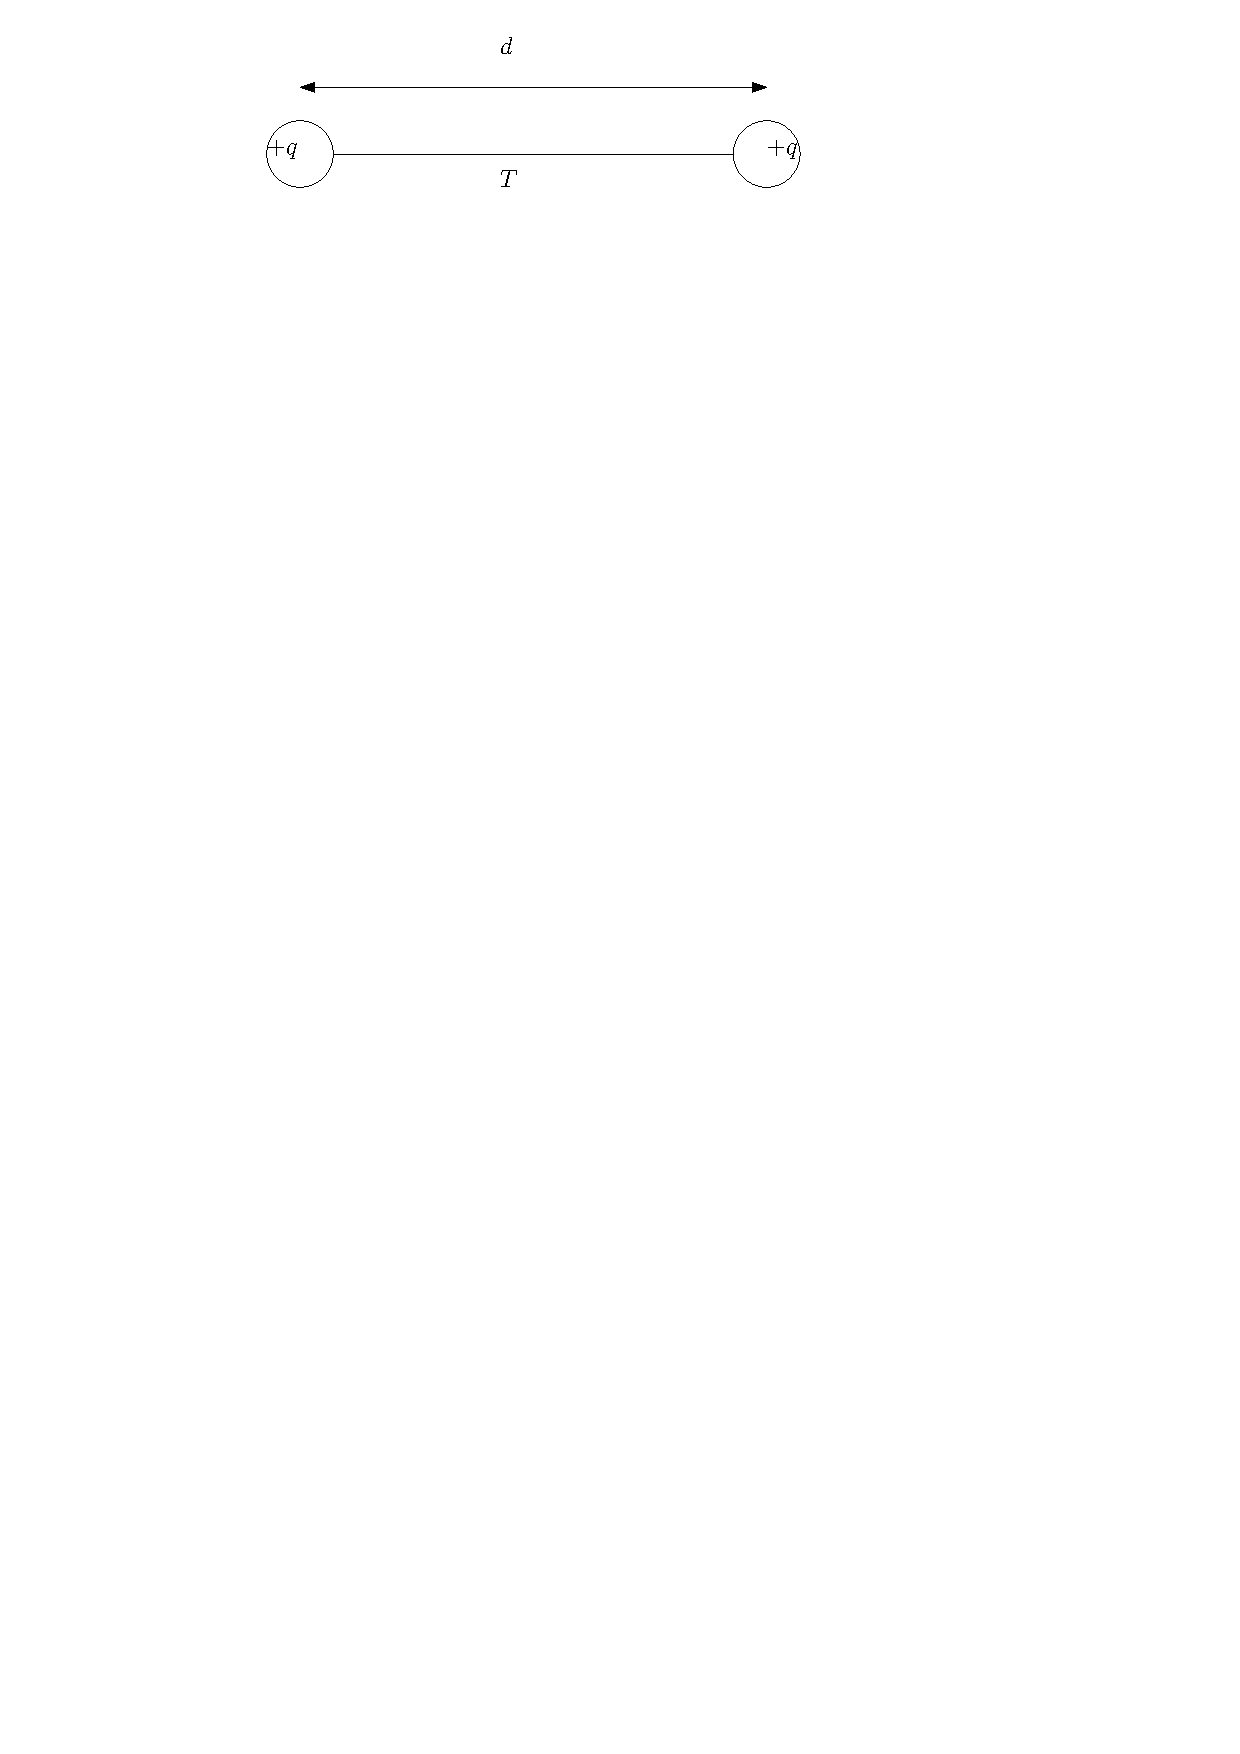
\includegraphics[width=0.5\textwidth]{2-charges.pdf}
\newpage
\noindent Consider the following charges that are attached by strings below.  Calculate the tensions, $T_1$ and $T_2$, between the charges.

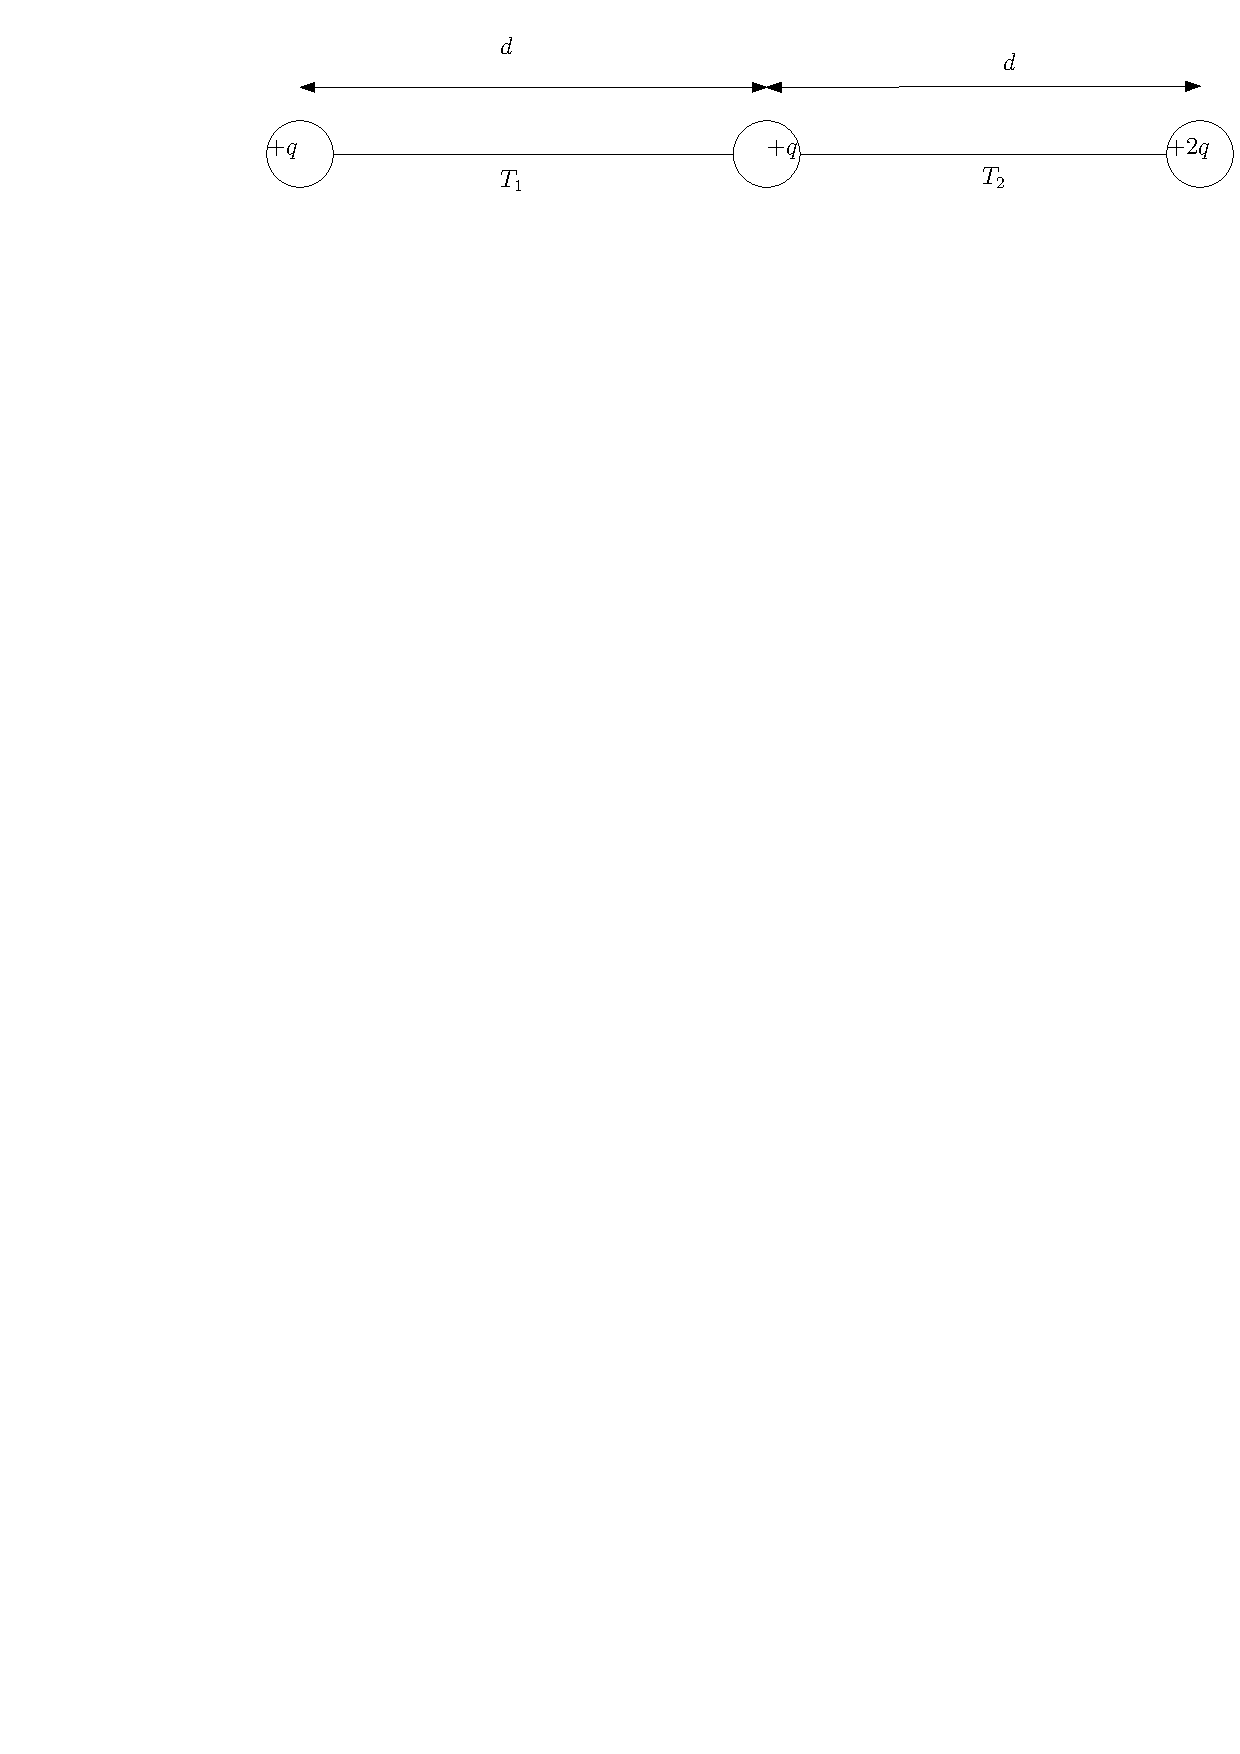
\includegraphics[width=0.75\textwidth]{3-charges.pdf}
\newpage 
\noindent Consider the following charges that are attached by rods below.  Calculate the forces, $F_1$ and $F_2$, between the charges.  What is the direction of each force? 

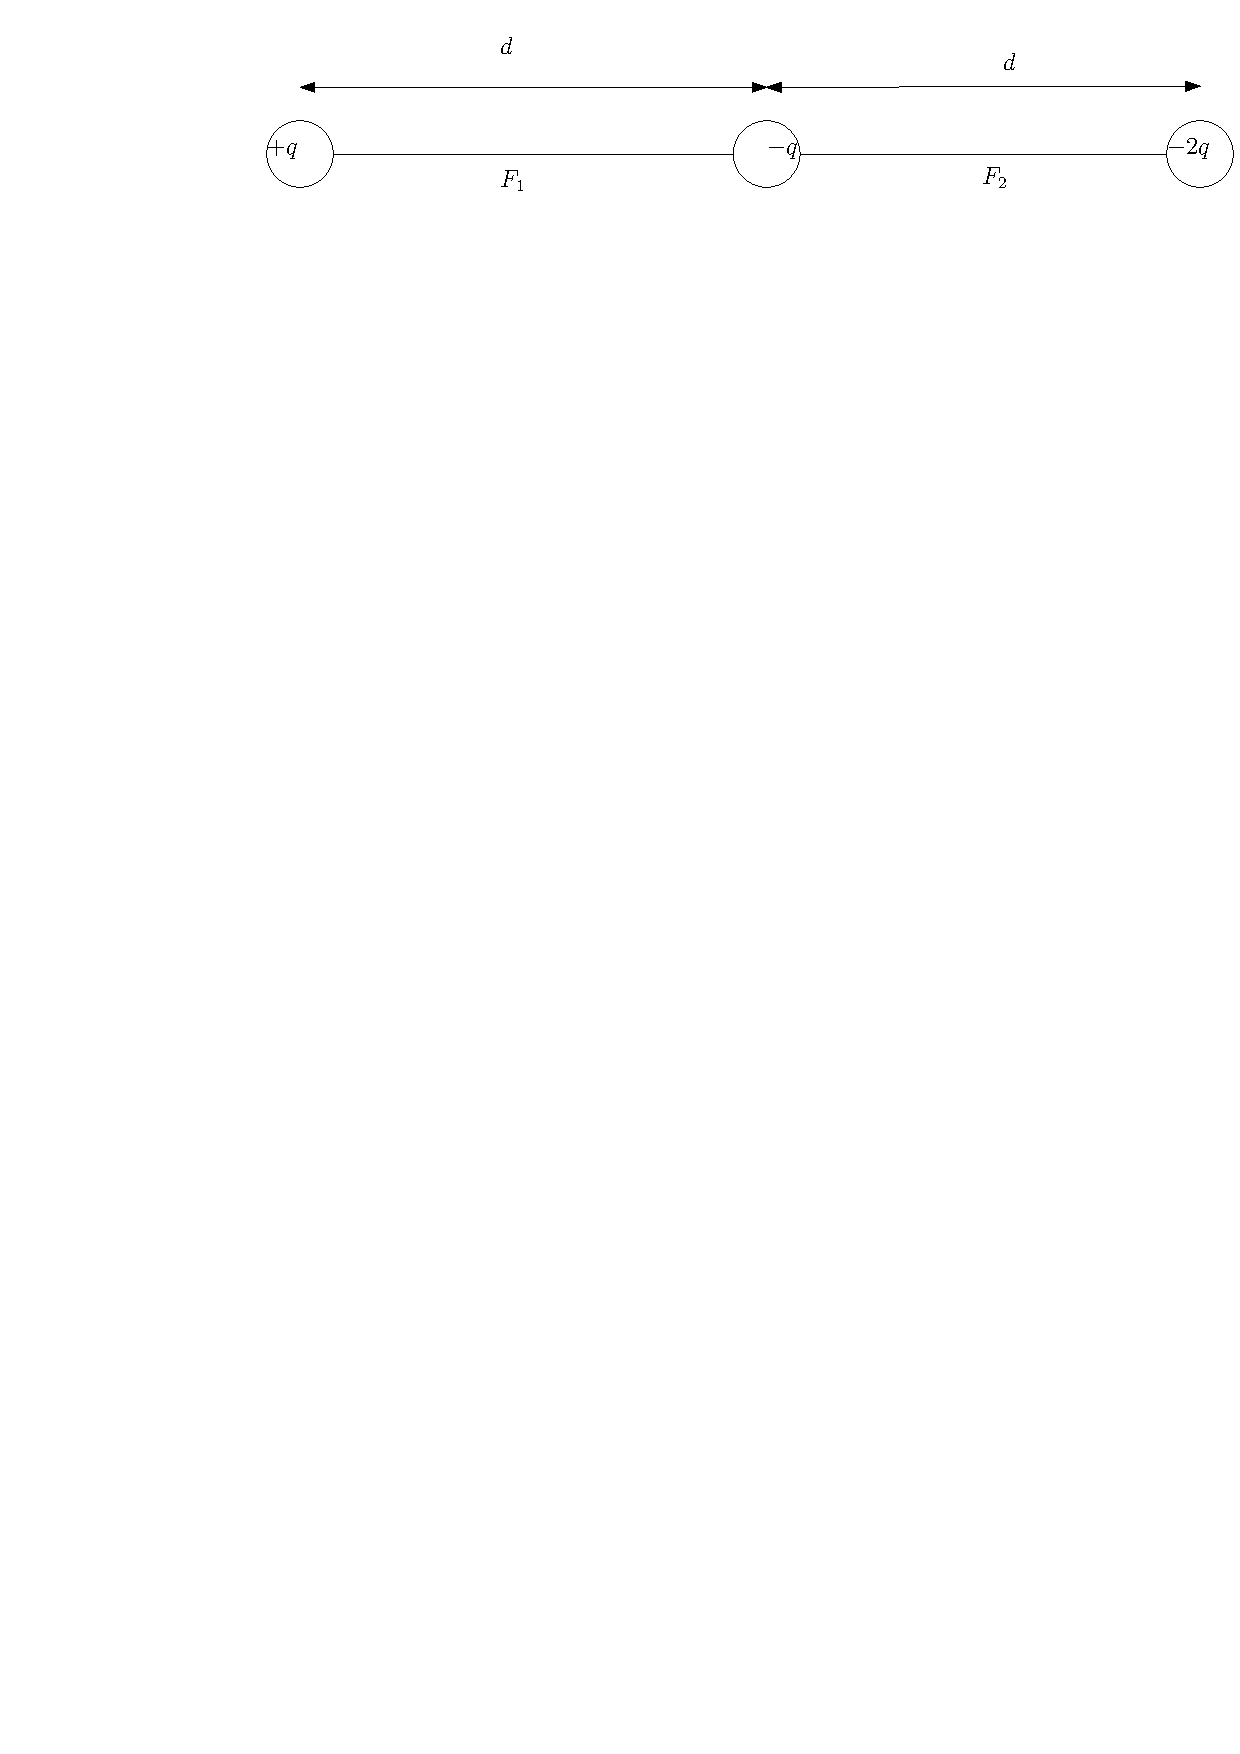
\includegraphics[width=0.75\textwidth]{3-charges-2.pdf}

\newpage
\noindent Consider four identical point charges arrange in a square below.  Show that the electric field at the the midpoint of each side of the square points outward (from the center of the square) and calculate it magnitude.

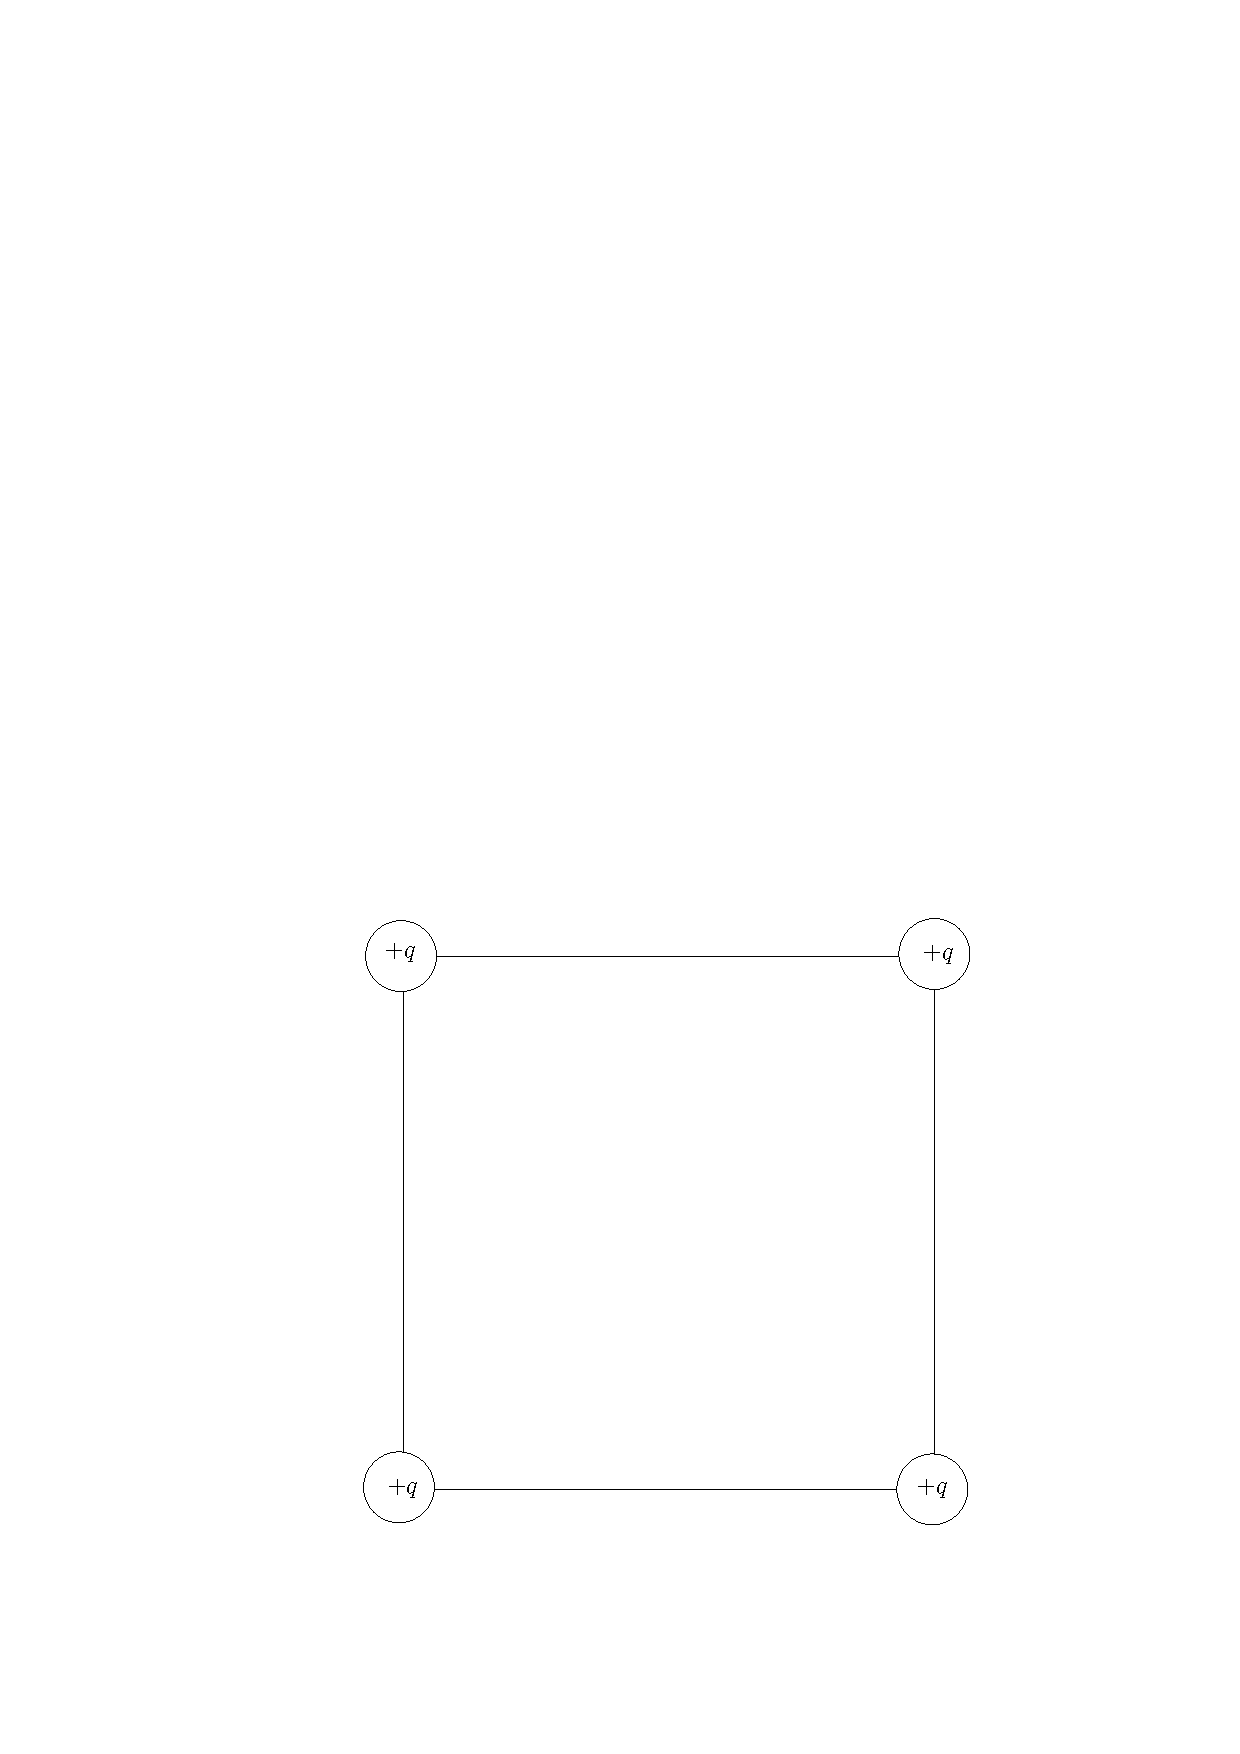
\includegraphics[width=0.25\textwidth]{square.pdf}

\newpage
\noindent A small test charge $+q$ and mass $m$ is constrained to move along the line connecting two charges, $+Q$, that are $d$ away on opposite sides.  Find the period of small oscillations.   
\newpage 
\noindent Consider a semi-infinite uniformly charged rod going from $x=0$ to $x=-\infty$.  What is the electric field in the x-direction at a point P whose coordinates are $(x,y)=(0,d)$? 
\newpage
\noindent Consider a semicircle (half a circle) with total charge Q and radius R as shown below.  What is the electric field at point $P$?

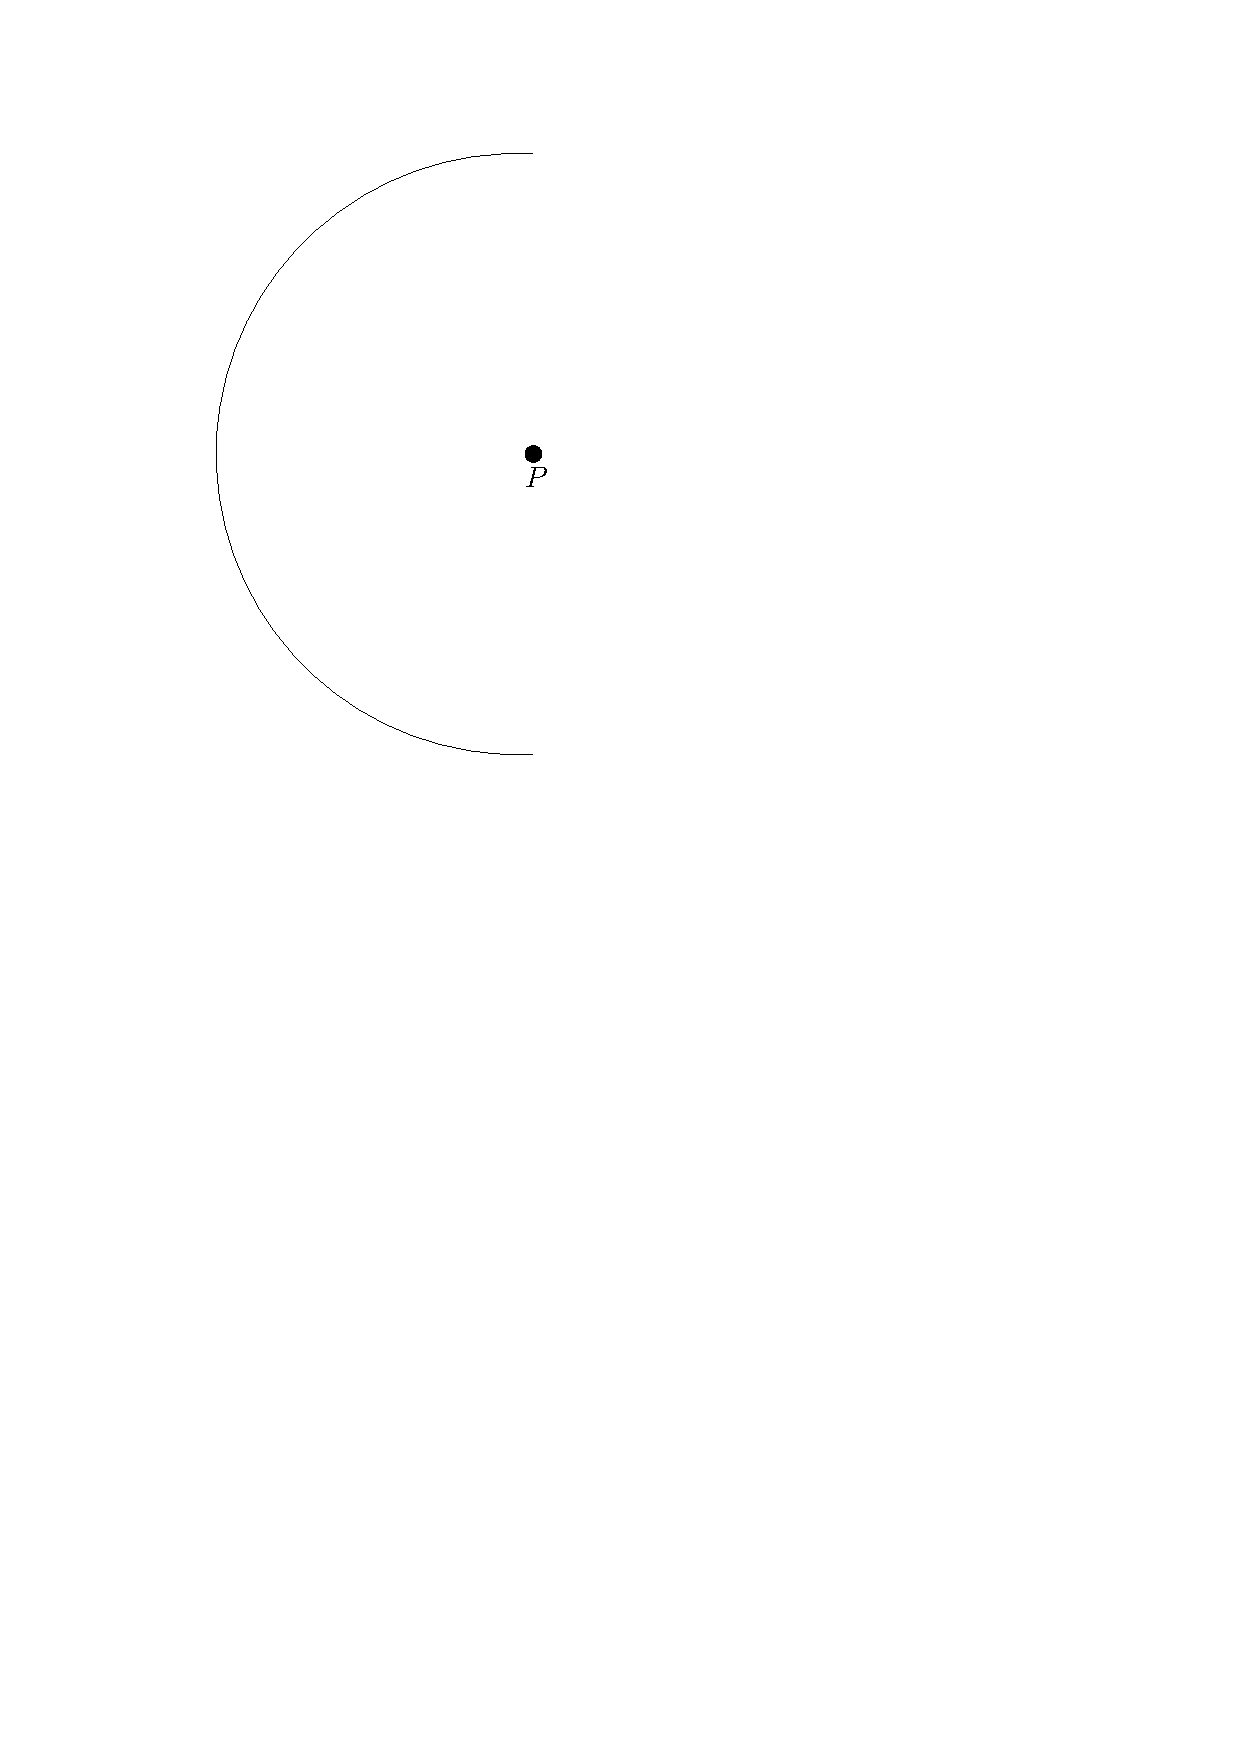
\includegraphics[width=0.12\textwidth]{semicircle.pdf}


\newpage
\noindent Consider a uniformed charged nonconducting sphere of total charge $Q$ and radius $R$.  Find an expression for the magnitude of the electric field as a function of $r$ for (a) $r>R$ and (b) $r\le R$.  How would these answers changes if the sphere was conducting?
\newpage
\noindent Consider the following model the hydrogen atom.  A small point change of $+q$ is surrounded by a spherical distribution of negative charge of the form $\rho = \rho_0 \exp(-r/r_0)$.  Using the fact that hydrogen atom is neutral, find $\rho_0$ in terms of $q$ and $r_0$.
\newpage
\noindent A uniformly charged nonconducting sphere would have total charge $Q$ if it was a complete sphere.  However, someone has come along and hollowed it out as shown in the figure below.  Find the electric force at the point $P$.

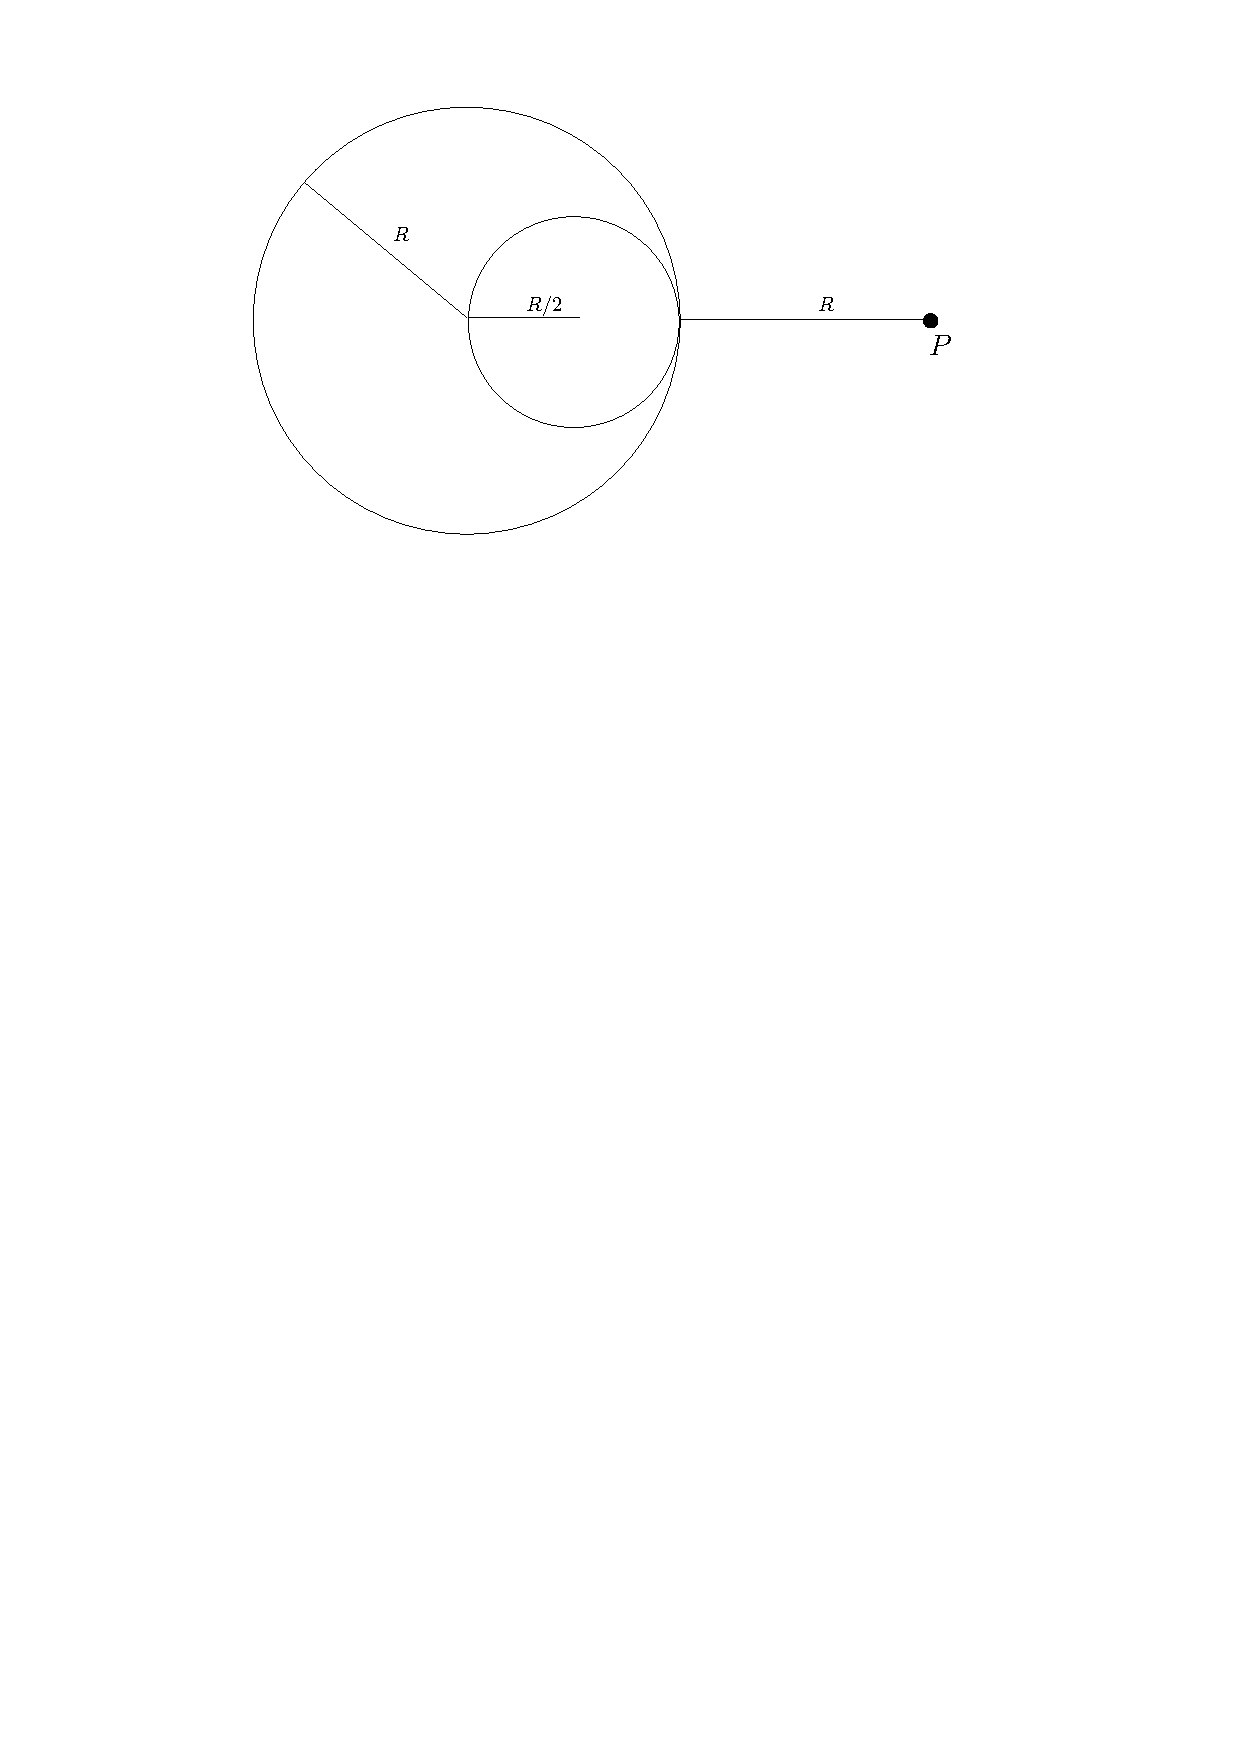
\includegraphics[width=0.35\textwidth]{sphere.pdf}

\newpage
\noindent A stationary ring of radius, $R$, has total charge $Q$.  A small particle of mass $m$ and charge $-q$ is constrained to move along the symmetry axis of the ring.  (a) Show that the center of the ring is an equilibrium point for the particle. (b) For small displacements around this equilibrium points, show that it executes simple harmonic motion and find the frequency.    
\newpage
\noindent An infinitely long conducting cylinder of radius $R$ has a charge per unit length of $\sigma$.  Find the electric field as a function of $r$.  
\end{document}
